\section{Results}
\subsection{Subjects}
Twelve healthy users (age $27 \pm 3.9$) participated in the experiment.  All
participants had normal, or corrected to normal vision, and reported not to use
medication. Only three of our subjects were female, and all subjects were
right-handed. Most participants had some video game experience, and four
subjects had previous experience with \acp{BCI}.

\subsection{Self assessments}
To verify the induction of changes in the mental state, we analysed the self
reported emotional ratings of the \ac{SAM}. Most subjects rated the \ac{LOC}
condition more negatively than the normal condition, over subjects this
difference was significant ($T$=3, $p$\textless 0.01). While we expected to
find a trend towards more arousal in the \ac{LOC} condition, there was no
significant difference ($T$=23, $p$=0.26). The dominance dimension, which
measures the amount of dominance, or control they have on their environment,
indicate that people seemed to be significantly ($T$=3.5, $p$\textless 0.01)
more in control in the normal condition.


\begin{figure}
  \center
  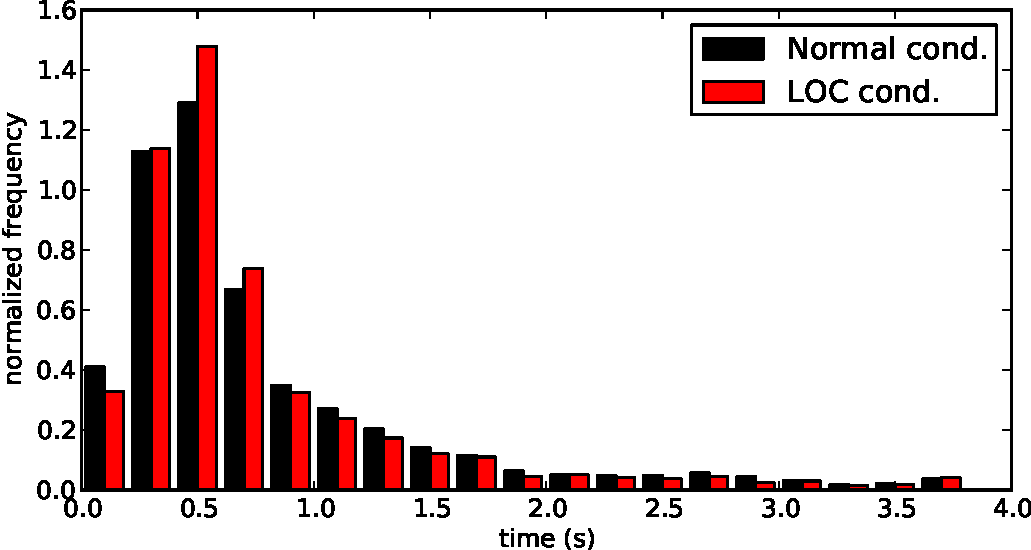
\includegraphics[width=3.5in]{key_duration.pdf}
  \caption{The histogram for the time between key presses during game play for
  all subjects. The intervals for the normal condition are displayed in black,
  the \protect\ac{LOC} condition is displayed in red (gray). The histogram is
  dominated by short $\Delta t$'s between key presses. The histogram of the
  \protect\ac{LOC} condition seems to be slightly more pinched around half a
  second.}
  \label{fig:key_duration}
\end{figure}

\begin{figure}
  \center
  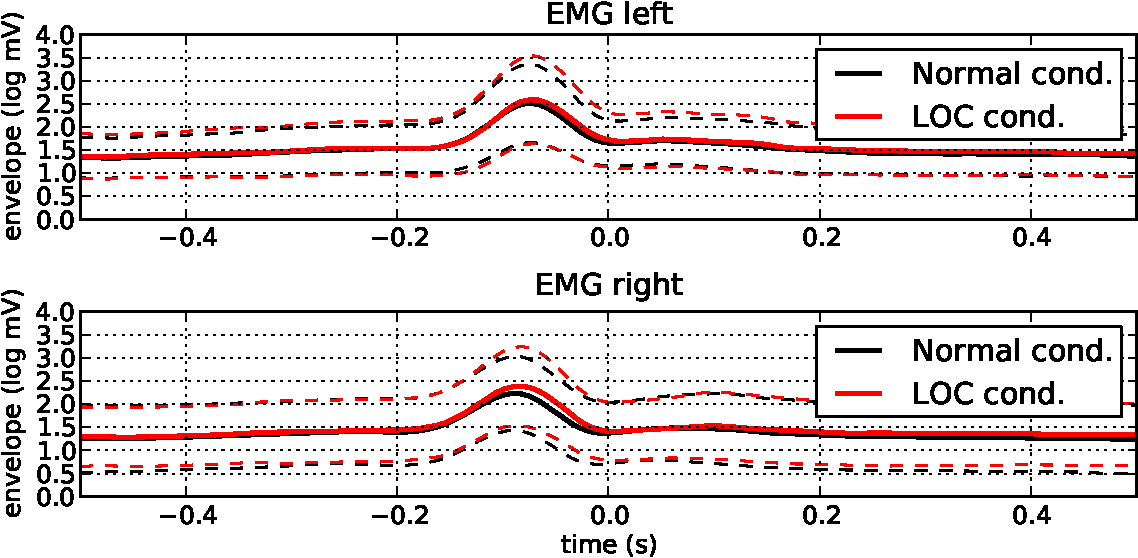
\includegraphics[width=3.5in]{emg_cond.pdf}
  \caption{The mean log \protect\ac{EMG} power and its standard deviation
  (dashed lines) is displayed for both the normal and \protect\ac{LOC}
  condition, time-locked to the key press at $t=0$. The top plot shows the EMG
  power of the left bipolar channel for left index-finger presses, the bottom
  plot show the EMG power for right hand movement measured with the right
  bipolar channel.}
  \label{fig:emg_cond}
\end{figure}

\begin{table}
  \caption{Statistics of confounding variables. The repetitiveness (second
  column) and log-\protect\ac{EMG} power (last column) differ significantly
  between the conditions. The \protect\ac{EMG} power was quantified as the
  maximum power in the interval [-0.2,~0]~s. The start and end of the arrow
  signify the mean value in the normal and \protect{LOC} condition
  respectively.} 
  \center \footnotesize
  \begin{tabular}{c c c c c}
\toprule
 & log $\Delta t$ & $p(y_t=y_{t-1})$ & log pow. EMG L & log pow. EMG R\\
\midrule
S0 & -0.48 $\rightarrow$ -0.36 &  0.51 $\rightarrow$  0.59 &  1.31 $\rightarrow$  1.21 &  1.08 $\rightarrow$  1.15\\
S1 & -0.51 $\rightarrow$ -0.53 &  0.54 $\rightarrow$  0.59 &  2.70 $\rightarrow$  2.60 &  2.04 $\rightarrow$  2.17\\
S2 & -0.54 $\rightarrow$ -0.59 &  0.50 $\rightarrow$  0.52 &  2.65 $\rightarrow$  2.58 &  2.51 $\rightarrow$  2.46\\
S3 & -0.47 $\rightarrow$ -0.61 &  0.56 $\rightarrow$  0.54 &  1.99 $\rightarrow$  1.88 &  2.15 $\rightarrow$  2.31\\
S4 & -0.46 $\rightarrow$ -0.55 &  0.53 $\rightarrow$  0.58 &  3.14 $\rightarrow$  3.35 &  1.76 $\rightarrow$  1.86\\
S5 & -0.46 $\rightarrow$ -0.44 &  0.56 $\rightarrow$  0.60 &  2.70 $\rightarrow$  2.56 &  4.06 $\rightarrow$  3.91\\
S6 & -0.46 $\rightarrow$ -0.48 &  0.55 $\rightarrow$  0.55 &  2.11 $\rightarrow$  2.55 &  2.14 $\rightarrow$  2.47\\
S7 & -0.40 $\rightarrow$ -0.55 &  0.58 $\rightarrow$  0.56 &  1.70 $\rightarrow$  1.71 &  2.13 $\rightarrow$  2.14\\
S8 & -0.37 $\rightarrow$ -0.44 &  0.47 $\rightarrow$  0.56 &  2.89 $\rightarrow$  2.95 &  2.94 $\rightarrow$  3.02\\
S9 & -0.58 $\rightarrow$ -0.55 &  0.45 $\rightarrow$  0.54 &  3.02 $\rightarrow$  3.08 &  2.01 $\rightarrow$  2.06\\
S10 & -0.58 $\rightarrow$ -0.44 &  0.47 $\rightarrow$  0.53 &  2.43 $\rightarrow$  2.42 &  2.52 $\rightarrow$  2.55\\
S11 & -0.45 $\rightarrow$ -0.42 &  0.52 $\rightarrow$  0.58 &  3.01 $\rightarrow$  2.86 &  2.97 $\rightarrow$  3.13\\
\midrule
mean & -0.48 $\rightarrow$ -0.50 &  0.52 $\rightarrow$  0.56 &  2.47 $\rightarrow$  2.48 &  2.36 $\rightarrow$  2.44\\
Wilc. & T=32, p=0.583 & \textbf{T=6, p=0.010} & T=31, p=0.530 & \textbf{T=12, p=0.034}\\
\bottomrule
\end{tabular}

  \label{tab:confounds} 
\end{table}

\subsection{Confounding behavioural differences} \label{sec:behav} 
In this section we describe the analysis of the characteristics of the user's
behaviour, as it might have had a confounding influence on the \ac{BCI}
performance. 
%
Both differences in the \ac{ITI}, and the pattern of consecutive keystrokes
can indicate a confounding behavioural change. The per-subject statistics for
these confounding factors are presented in Table~\ref{tab:confounds}. For the
log \ac{ITI}, we see an insignificant tendency to shorter intervals between key
presses in the \ac{LOC} condition. The probability that a key press was made
with the same hand is significantly higher in the \ac{LOC} condition. This may have been caused by increased repetition, by increased imbalance of the class ratios,
or a combination thereof. Nevertheless, it indicates a significant behavioural
change.

The temporal development of the \ac{EMG} signal is displayed in
Fig.~\ref{fig:emg_cond}. An increase in the \ac{EMG} power is visible just
before the stroke is registered, and a much weaker increase is visible when the
key is released. Most of the activity is registered in the interval [-0.2, 0]~s
relative to the registration of the key press. We used the maximum \ac{EMG}
power in this interval to estimate the force used to press a key (see
Table~\ref{tab:confounds}). Movements with the right index finger produce
significantly more \ac{EMG} power in the \ac{LOC} condition.

\begin{figure}
  \center
  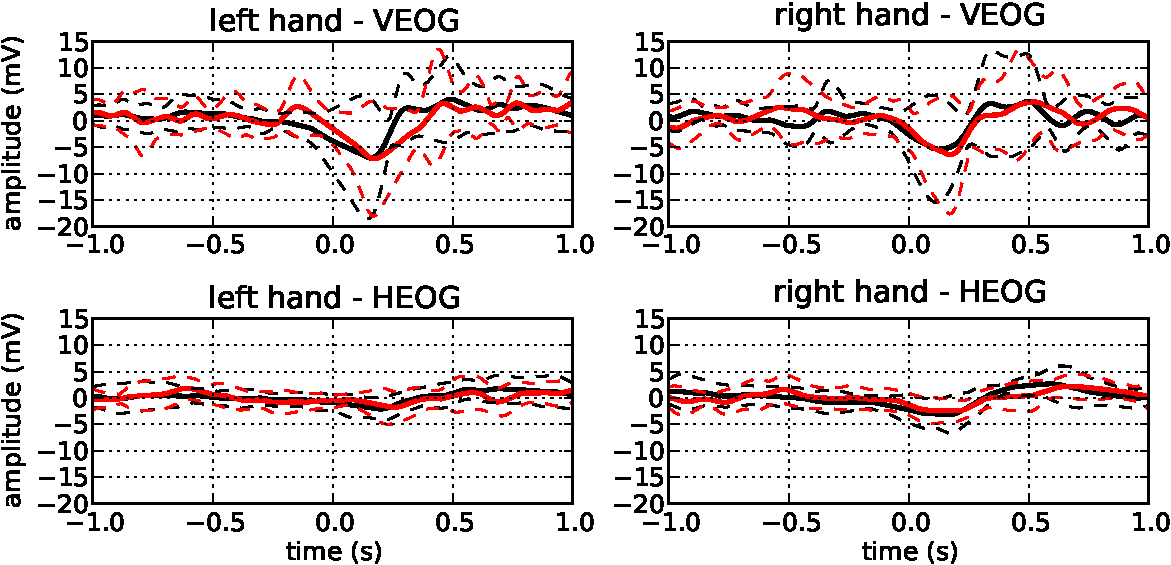
\includegraphics[width=\textwidth]{eog_cond.pdf}
  \caption{The vertical eye movement (first row) show downward eye-gaze just
  after a keystroke at $t=0$. The horizontal bipolar \protect\ac{EOG} channel
  is rather uneventful, only for right hand movement (last column) does there
  appear to be a delayed reaction to the key press, first negative (looking
  left) then positive (looking right). The dashed lines indicate the standard
  deviation.  There is no significant difference (16 point Bonferroni corrected
  Wilcoxon signed-rank test over subjects) between the normal (black) and
  \protect\ac{LOC} condition (red).}
  \label{fig:eog_cond}
\end{figure}

Although we removed (most) of the influence of the \ac{EOG} signal from the
\ac{EEG}, it is interesting to look at the user's gaze and blink behaviour
during a key press (Fig.~\ref{fig:eog_cond}). We can see that users tend to
look at their hands 200~ms after a key press, which is most visible in the
vertical \ac{EOG}, and at 300~ms, the variability of the vertical \ac{EOG}
signal seems to increase. This might be caused by eye-blinks, or an adjustment
to the new movement direction of the avatar in the game. 

In summary, our behaviour analysis has shown that the normal and
\ac{LOC}-con\-di\-tions are very similar in the timing, the predictability of
the key\-strokes, the amount of force used to press the keys, and in eye
movements. However, there was a small but significant increase in repetition of
the same movement, and a small significant increase in the force used with the
right hand. After balancing the confounding variables and their interactions
per subject, on average 25\% of the original trials were removed.

\subsection{Impact of loss of control on the BCI}
To investigate the influence of \ac{LOC} on the \ac{BCI} performance, we
trained the \ac{ERD} based and the \ac{ERP}-based classifier on blocks from the
normal condition, and compared the performance on unseen normal blocks with the
performance on blocks from the \ac{LOC} condition. Please refer to
Section~\ref{sec:dga} for more information on this procedure.

\begin{table*} 
  \caption{The influence of \protect\ac{LOC} on a \protect\ac{CSP} classifier
  is shown below, without correction for confounding factors. The start and end
  of the arrow indicate the median performance for the normal and
  \protect\ac{LOC} condition respectively. The $p$-value of a Mann-Whitney U
  test on the per-block performance is displayed above the arrow. The row
  denoted with ``Wilc.'' signifies the over-subject comparison with the Wilcoxon
  signed rank test. The row denoted by ``Fish.'' presents the results of
  combining one-sided $p$-values for an increase in performance.}
  \center \scriptsize
  \begin{tabular}{c c c c c}
\toprule
 & Accuracy & AUC & MI & ITR\\
\midrule
S0 &  0.679 $\xrightarrow{p=0.35}$  0.736 &  0.759 $\xrightarrow{p=0.35}$  0.843 &  0.110 $\xrightarrow{p=0.35}$  0.193 & 11.680 $\xrightarrow{p=0.48}$ 13.763\\
S1 &  0.599 $\xrightarrow{p=0.48}$  0.618 &  0.616 $\xrightarrow{p=0.64}$  0.652 &  0.021 $\xrightarrow{p=0.64}$  0.041 &  2.601 $\xrightarrow{p=0.64}$  4.525\\
S2 &  0.619 $\xrightarrow{p=0.92}$  0.555 &  0.543 $\xrightarrow{p=0.62}$  0.578 &  0.001 $\xrightarrow{p=0.77}$  0.000 &  0.088 $\xrightarrow{p=0.92}$  0.025\\
S3 &  0.474 $\xrightarrow{p=0.13}$  0.519 & \textbf{ 0.466 $\xrightarrow{p=0.05}$  0.518} &  0.004 $\xrightarrow{p=0.62}$  0.003 &  0.452 $\xrightarrow{p=0.77}$  0.338\\
S4 &  0.519 $\xrightarrow{p=0.92}$  0.507 &  0.549 $\xrightarrow{p=0.92}$  0.526 &  0.002 $\xrightarrow{p=0.77}$  0.003 &  0.224 $\xrightarrow{p=0.77}$  0.351\\
S5 &  0.741 $\xrightarrow{p=0.92}$  0.750 &  0.828 $\xrightarrow{p=0.92}$  0.832 &  0.167 $\xrightarrow{p=0.92}$  0.188 & 15.616 $\xrightarrow{p=0.92}$ 20.297\\
S6 &  0.538 $\xrightarrow{p=0.65}$  0.529 &  0.543 $\xrightarrow{p=0.86}$  0.522 &  0.003 $\xrightarrow{p=0.59}$  0.006 &  0.302 $\xrightarrow{p=0.59}$  0.664\\
S7 &  0.544 $\xrightarrow{p=0.10}$  0.600 &  0.565 $\xrightarrow{p=0.27}$  0.657 &  0.005 $\xrightarrow{p=0.19}$  0.027 &  0.532 $\xrightarrow{p=0.08}$  3.082\\
S8 &  0.542 $\xrightarrow{p=0.34}$  0.581 &  0.556 $\xrightarrow{p=0.34}$  0.589 &  0.004 $\xrightarrow{p=0.48}$  0.010 &  0.366 $\xrightarrow{p=0.48}$  1.035\\
S9 &  0.735 $\xrightarrow{p=0.15}$  0.768 &  0.797 $\xrightarrow{p=0.15}$  0.839 &  0.160 $\xrightarrow{p=0.15}$  0.218 & 18.879 $\xrightarrow{p=0.15}$ 24.494\\
S10 &  0.612 $\xrightarrow{p=0.35}$  0.582 &  0.670 $\xrightarrow{p=0.48}$  0.651 &  0.046 $\xrightarrow{p=0.35}$  0.018 &  5.611 $\xrightarrow{p=0.35}$  2.108\\
S11 &  0.608 $\xrightarrow{p=0.34}$  0.553 &  0.594 $\xrightarrow{p=0.95}$  0.599 &  0.020 $\xrightarrow{p=0.95}$  0.023 &  2.371 $\xrightarrow{p=0.64}$  2.059\\
\midrule
mean & 0.601 $\rightarrow$ 0.608 & 0.624 $\rightarrow$ 0.651 & 0.045 $\rightarrow$ 0.061 & 4.893 $\rightarrow$ 6.062\\
Wilc. & T=31.0, p=0.530 & \textbf{T=12.0, p=0.034} & \textbf{T=14.0, p=0.050} & T=17.0, p=0.084\\
%Fish. 2-way & p=0.469 & p=0.643 & p=0.846 & p=0.793\\
Fish. & p=0.123 & p=0.078 & p=0.259 & p=0.222\\
%Fish. 1-way - & p=0.912 & p=0.986 & p=0.947 & p=0.941\\
\bottomrule
\end{tabular}

  \label{tab:csp}
\end{table*}

\begin{table*} 
  \caption{The influence of \protect\ac{LOC} on a \protect\ac{CSP} classifier
  is shown below, with correction for confounding factors enabled. Please refer
  to Table~\ref{tab:csp} for an explanation. } 
  \center \scriptsize
  \begin{tabular}{c c c c c}
\toprule
 & Accuracy & AUC & MI & ITR\\
\midrule
S0 &  0.678 $\xrightarrow{p=0.64}$  0.667 &  0.718 $\xrightarrow{p=0.35}$  0.785 &  0.094 $\xrightarrow{p=0.82}$  0.056 &  7.370 $\xrightarrow{p=0.95}$  4.896\\
S1 & \textbf{ 0.543 $\xrightarrow{p=0.05}$  0.646} &  0.572 $\xrightarrow{p=0.09}$  0.686 & \textbf{ 0.007 $\xrightarrow{p=0.05}$  0.063} &  0.734 $\xrightarrow{p=0.09}$  6.751\\
S2 &  0.640 $\xrightarrow{p=1.00}$  0.626 &  0.558 $\xrightarrow{p=0.92}$  0.548 &  0.009 $\xrightarrow{p=0.19}$  0.002 &  0.825 $\xrightarrow{p=0.27}$  0.165\\
S3 &  0.541 $\xrightarrow{p=0.62}$  0.553 &  0.483 $\xrightarrow{p=0.62}$  0.514 &  0.007 $\xrightarrow{p=0.77}$  0.005 &  0.482 $\xrightarrow{p=0.62}$  0.450\\
S4 &  0.569 $\xrightarrow{p=0.19}$  0.532 &  0.572 $\xrightarrow{p=0.77}$  0.536 &  0.013 $\xrightarrow{p=0.92}$  0.008 &  1.416 $\xrightarrow{p=0.92}$  0.769\\
S5 &  0.753 $\xrightarrow{p=0.77}$  0.743 &  0.857 $\xrightarrow{p=0.62}$  0.821 &  0.198 $\xrightarrow{p=0.77}$  0.180 & 14.086 $\xrightarrow{p=0.77}$ 15.423\\
S6 &  0.532 $\xrightarrow{p=0.21}$  0.558 & \textbf{ 0.498 $\xrightarrow{p=0.01}$  0.579} &  0.004 $\xrightarrow{p=0.10}$  0.011 &  0.308 $\xrightarrow{p=0.06}$  0.874\\
S7 &  0.549 $\xrightarrow{p=0.37}$  0.577 &  0.613 $\xrightarrow{p=0.92}$  0.623 &  0.010 $\xrightarrow{p=0.49}$  0.015 &  0.964 $\xrightarrow{p=0.37}$  1.534\\
S8 &  0.543 $\xrightarrow{p=0.48}$  0.605 &  0.549 $\xrightarrow{p=0.23}$  0.583 & \textbf{ 0.002 $\xrightarrow{p=0.02}$  0.017} & \textbf{ 0.166 $\xrightarrow{p=0.02}$  1.394}\\
S9 &  0.687 $\xrightarrow{p=0.23}$  0.740 &  0.783 $\xrightarrow{p=0.23}$  0.833 &  0.086 $\xrightarrow{p=0.15}$  0.162 &  8.770 $\xrightarrow{p=0.15}$ 16.045\\
S10 & \textbf{ 0.658 $\xrightarrow{p=0.05}$  0.617} &  0.676 $\xrightarrow{p=0.82}$  0.673 &  0.054 $\xrightarrow{p=0.24}$  0.035 &  4.888 $\xrightarrow{p=0.35}$  3.147\\
S11 &  0.585 $\xrightarrow{p=0.23}$  0.551 & \textbf{ 0.615 $\xrightarrow{p=0.01}$  0.544} &  0.021 $\xrightarrow{p=0.23}$  0.005 &  1.329 $\xrightarrow{p=0.15}$  0.366\\
\midrule
mean & 0.606 $\rightarrow$ 0.618 & 0.625 $\rightarrow$ 0.644 & 0.042 $\rightarrow$ 0.047 & 3.445 $\rightarrow$ 4.318\\
Wilc. & T=31.0, p=0.530 & T=27.0, p=0.347 & T=35.0, p=0.754 & T=35.0, p=0.754\\
%Fish. 2-way & p=0.172 & p=0.077 & p=0.081 & p=0.083\\
Fish. & p=0.237 & \textbf{p=0.050} & p=0.063 & \textbf{p=0.047}\\
%Fish. 1-way - & p=0.443 & p=0.602 & p=0.622 & p=0.707\\
\bottomrule
\end{tabular}

  \label{tab:csp_bal}
\end{table*}

The performance of the \ac{CSP} based features classifier on the normal and
\ac{LOC} blocks without correction for confounds is displayed in
Table~\ref{tab:csp}. The single trial detection accuracy may seem rather low
(60\%), but this is similar to the accuracies obtained in other studies that
use short \acp{ITI}, such as \cite{jatzev2008ecn}. This was also reflected in
the mean \ac{ITR} of 5.5 bits per minute, which is comparable to the \acp{ITR}
obtained by naive users with motor-imagery based \ac{ERD} \acp{BCI}.
%
Despite this low recognition rate, the \ac{ERD} \acp{BCI} performance did
significantly \emph{increase} in the \ac{LOC} condition for the \ac{AUC} and
\ac{MI} measures.

When correction for confounding factors was performed, the results were
different (Table~\ref{tab:csp_bal}); the over-subject differences disappeared,
but there were more significant within-subject differences in sometimes opposing
directions. Combined with Fisher's method, the one-sided $p$-values for a
within-subject increase in performance was significant for both \ac{AUC} and
\ac{ITR}. This indicates at least one individual increase in performance was
significant at the $\alpha=0.05$ level.

\begin{sidewaysfigure}
  \centering
  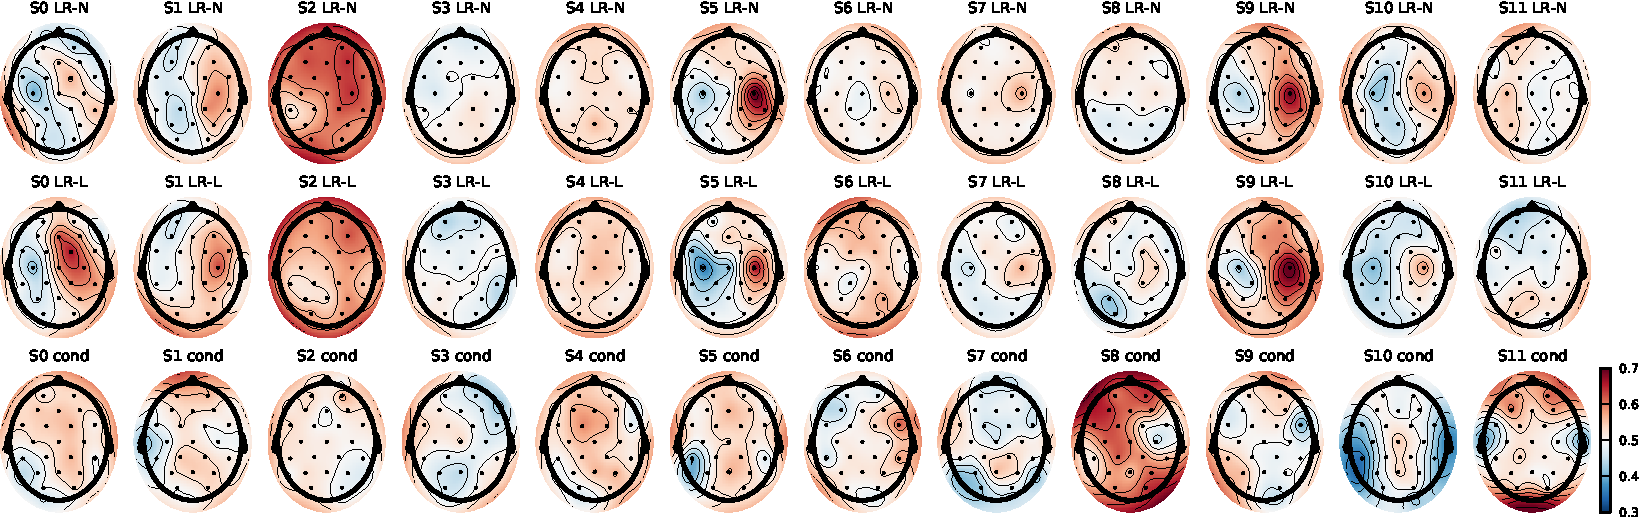
\includegraphics[width=\textwidth]{figs/bp_nlc.pdf}
  \caption{
  These scalp plots display the difference between left and right hand movement
  in the normal (first row) and \protect\ac{LOC} condition (second row), and
  the difference between the normal and \protect\ac{LOC} in the last row. 
  %
  The color encodes the \protect\ac{AUC}-\protect\ac{ROC} ranking performance
  of the 8--30~Hz band power at the specified location; red indicates a
  positive rank correlation with the target class (right hand for the first two
  rows, or \protect\ac{LOC} in the last), blue a negative correlation. The
  conditions were corrected for confounding factors with frequency matching.
  %
  Most subjects display a more pronounced spatial activation in
  the \protect\ac{LOC} condition.}
  \label{fig:ERD_diff} 
\end{sidewaysfigure}

\begin{sloppypar}
The spatial distribution of the movement related \ac{ERD} is shown in
Fig.~\ref{fig:ERD_diff}. Subjects S0, S1, S5,  S9 and S10 do display the
prototypical \ac{ERD} on the motor cortices. Remarkably, these activations are
more pronounced in the \ac{LOC} condition (second row), which supports the
observed increase in performance. 
%
Note that the \ac{CSP} classification is based on covariance of the \ac{EEG}
channels, while in this figure only the variance is shown. 
\end{sloppypar}


\begin{table*}
  \caption{The influence of \protect\ac{LOC} on a \protect\ac{ERP} classifier
  is shown below, without correction for confounding factors. Please refer to
  Table~\ref{tab:csp} for an explanation.}
  \center \scriptsize
  \begin{tabular}{c c c c c}
\toprule
 & Accuracy & AUC & MI & ITR\\
\midrule
S0 &  0.765 $\xrightarrow{p=0.73}$  0.747 &  0.824 $\xrightarrow{p=0.95}$  0.812 &  0.223 $\xrightarrow{p=0.64}$  0.179 & 24.349 $\xrightarrow{p=0.48}$ 17.575\\
S1 &  0.802 $\xrightarrow{p=0.34}$  0.758 &  0.866 $\xrightarrow{p=0.64}$  0.823 &  0.282 $\xrightarrow{p=0.23}$  0.195 & 32.838 $\xrightarrow{p=0.34}$ 22.092\\
S2 &  0.726 $\xrightarrow{p=0.27}$  0.750 &  0.790 $\xrightarrow{p=0.49}$  0.809 &  0.142 $\xrightarrow{p=0.62}$  0.154 & 16.269 $\xrightarrow{p=0.37}$ 18.677\\
S3 &  0.711 $\xrightarrow{p=0.77}$  0.724 &  0.779 $\xrightarrow{p=0.62}$  0.788 &  0.133 $\xrightarrow{p=0.77}$  0.139 & 11.719 $\xrightarrow{p=0.77}$ 16.195\\
S4 &  0.692 $\xrightarrow{p=0.92}$  0.714 &  0.767 $\xrightarrow{p=0.37}$  0.803 &  0.096 $\xrightarrow{p=0.92}$  0.110 & 11.672 $\xrightarrow{p=0.77}$ 11.882\\
S5 &  0.720 $\xrightarrow{p=0.77}$  0.715 &  0.800 $\xrightarrow{p=0.92}$  0.790 &  0.142 $\xrightarrow{p=0.92}$  0.136 & 14.584 $\xrightarrow{p=0.62}$ 15.041\\
S6 &  0.703 $\xrightarrow{p=0.15}$  0.726 &  0.766 $\xrightarrow{p=0.15}$  0.789 &  0.116 $\xrightarrow{p=0.10}$  0.155 & 13.460 $\xrightarrow{p=0.10}$ 16.812\\
S7 &  0.772 $\xrightarrow{p=0.77}$  0.778 &  0.833 $\xrightarrow{p=0.62}$  0.857 &  0.225 $\xrightarrow{p=0.77}$  0.234 & 23.515 $\xrightarrow{p=0.62}$ 26.844\\
S8 &  0.702 $\xrightarrow{p=0.64}$  0.742 & \textbf{ 0.778 $\xrightarrow{p=0.05}$  0.830} &  0.121 $\xrightarrow{p=0.64}$  0.175 & 10.529 $\xrightarrow{p=0.23}$ 18.768\\
S9 &  0.831 $\xrightarrow{p=0.48}$  0.785 &  0.886 $\xrightarrow{p=0.34}$  0.873 &  0.328 $\xrightarrow{p=0.48}$  0.246 & 38.768 $\xrightarrow{p=0.34}$ 29.488\\
S10 &  0.704 $\xrightarrow{p=0.82}$  0.701 &  0.790 $\xrightarrow{p=0.95}$  0.783 &  0.129 $\xrightarrow{p=0.82}$  0.120 & 14.146 $\xrightarrow{p=0.95}$ 14.663\\
S11 &  0.835 $\xrightarrow{p=0.81}$  0.843 &  0.931 $\xrightarrow{p=0.81}$  0.921 &  0.344 $\xrightarrow{p=0.64}$  0.375 & 41.528 $\xrightarrow{p=0.81}$ 38.285\\
\midrule
mean & 0.747 $\rightarrow$ 0.749 & 0.818 $\rightarrow$ 0.823 & 0.190 $\rightarrow$ 0.185 & 21.115 $\rightarrow$ 20.5\\
Wilc. & T=32.0, p=0.583 & T=30.0, p=0.480 & T=36.0, p=0.814 & T=37.0, p=0.875\\
%Fish. 2-way & p=0.943 & p=0.745 & p=0.936 & p=0.765\\
Fish. & p=0.546 & p=0.197 & p=0.570 & p=0.350\\
%Fish. 1-way - & p=0.825 & p=0.927 & p=0.786 & p=0.842\\
\bottomrule
\end{tabular}

  \label{tab:wherp}
\end{table*}

\begin{table*}
  \caption{The influence of \protect\ac{LOC} on a \protect\ac{ERP} classifier
  is shown below, with correction for confounding factors enabled. Please refer
  to Table~\ref{tab:csp} for an explanation.}
  \center \scriptsize
  \begin{tabular}{c c c c c}
\toprule
 & Accuracy & AUC & MI & ITR\\
\midrule
S0 &  0.710 $\xrightarrow{p=0.35}$  0.732 &  0.800 $\xrightarrow{p=0.64}$  0.820 &  0.134 $\xrightarrow{p=0.48}$  0.164 & 11.145 $\xrightarrow{p=0.95}$  9.779\\
S1 &  0.810 $\xrightarrow{p=0.15}$  0.777 &  0.870 $\xrightarrow{p=0.48}$  0.854 &  0.295 $\xrightarrow{p=0.15}$  0.233 & 28.990 $\xrightarrow{p=0.23}$ 19.258\\
S2 &  0.720 $\xrightarrow{p=0.92}$  0.746 &  0.792 $\xrightarrow{p=0.77}$  0.801 &  0.121 $\xrightarrow{p=0.62}$  0.127 & 12.031 $\xrightarrow{p=0.77}$ 12.806\\
S3 &  0.716 $\xrightarrow{p=0.77}$  0.702 &  0.763 $\xrightarrow{p=0.62}$  0.766 &  0.133 $\xrightarrow{p=0.92}$  0.134 &  9.135 $\xrightarrow{p=0.27}$ 11.983\\
S4 &  0.696 $\xrightarrow{p=0.62}$  0.707 &  0.759 $\xrightarrow{p=0.77}$  0.787 &  0.110 $\xrightarrow{p=0.77}$  0.133 & 12.860 $\xrightarrow{p=0.37}$ 13.445\\
S5 &  0.640 $\xrightarrow{p=0.77}$  0.649 &  0.729 $\xrightarrow{p=0.92}$  0.735 &  0.094 $\xrightarrow{p=0.27}$  0.071 &  7.364 $\xrightarrow{p=0.92}$  6.853\\
S6 &  0.671 $\xrightarrow{p=0.47}$  0.695 &  0.769 $\xrightarrow{p=0.86}$  0.760 &  0.086 $\xrightarrow{p=0.47}$  0.124 &  6.197 $\xrightarrow{p=0.72}$  7.992\\
S7 &  0.739 $\xrightarrow{p=0.92}$  0.733 &  0.824 $\xrightarrow{p=0.77}$  0.811 &  0.174 $\xrightarrow{p=0.92}$  0.164 & 15.149 $\xrightarrow{p=0.92}$ 15.587\\
S8 & \textbf{ 0.709 $\xrightarrow{p=0.05}$  0.799} & \textbf{ 0.777 $\xrightarrow{p=0.02}$  0.847} & \textbf{ 0.106 $\xrightarrow{p=0.05}$  0.265} & \textbf{ 9.679 $\xrightarrow{p=0.02}$ 21.099}\\
S9 &  0.845 $\xrightarrow{p=0.34}$  0.803 &  0.925 $\xrightarrow{p=0.23}$  0.874 &  0.379 $\xrightarrow{p=0.48}$  0.278 & 35.293 $\xrightarrow{p=0.34}$ 29.589\\
S10 &  0.671 $\xrightarrow{p=0.82}$  0.688 &  0.764 $\xrightarrow{p=0.95}$  0.765 &  0.089 $\xrightarrow{p=0.82}$  0.099 &  7.261 $\xrightarrow{p=0.35}$  9.269\\
S11 &  0.835 $\xrightarrow{p=0.81}$  0.822 &  0.921 $\xrightarrow{p=0.34}$  0.883 &  0.350 $\xrightarrow{p=0.81}$  0.331 & 23.343 $\xrightarrow{p=0.64}$ 26.231\\
\midrule
mean & 0.730 $\rightarrow$ 0.738 & 0.808 $\rightarrow$ 0.809 & 0.173 $\rightarrow$ 0.177 & 14.871 $\rightarrow$ 15.3\\
Wilc. & T=31.0, p=0.530 & T=38.0, p=0.937 & T=36.0, p=0.814 & T=28.0, p=0.388\\
%Fish. 2-way & p=0.760 & p=0.802 & p=0.718 & p=0.592\\
Fish. & p=0.392 & p=0.484 & p=0.456 & p=0.162\\
%Fish. 1-way - & p=0.753 & p=0.679 & p=0.663 & p=0.894\\
\bottomrule
\end{tabular}

  \label{tab:wherp_bal}
\end{table*}

In contrast to the \ac{ERD} based classifiers, the \ac{ERP} classifiers had a
constant high performance with a minimum \ac{ITR} of 11.6 bits per minute.
Furthermore, they did not seem to behave differently in the \ac{LOC} 
condition, not with (Table~\ref{tab:wherp_bal}) and not without correction for
confounding factors (Table~\ref{tab:wherp}).
%
Visual inspection of the classifier's weights confirmed that the most
discriminative features were located on the motor cortices, that is to say, the
\ac{BCI} was based on brain activity.
%
The increase in performance for S8 is probably a false positive, since the
combination over subjects with Fisher's method is not significant.
